\documentclass[10pt,a4paper,twocolumn]{article}
\usepackage[a4paper,margin=17mm,columnsep=6mm]{geometry}
\usepackage[T1]{fontenc}
\usepackage{newtxtext,newtxmath}
\usepackage{microtype}
\usepackage{amsmath}
\usepackage{booktabs}
\usepackage{graphicx}
\usepackage{xcolor}
\usepackage[font=small,labelfont=bf,skip=4pt]{caption}
\usepackage{enumitem}
\usepackage[hidelinks]{hyperref}
\usepackage{tabularx}
\usepackage{array}
\setlist{nosep,leftmargin=*}
\graphicspath{{fig/}}
\newcommand{\Tab}[1]{\input{tab/tab_#1.tex}}
\newcommand{\NApAltEnd}{3}
\newcommand{\NApAltOver}{0}
\newcommand{\NApAltPitch}{10.3}
\newcommand{\NApConvDh}{59}
\newcommand{\NApConvPitchHi}{7.8}
\newcommand{\NApConvPitchLo}{$-$2.1}
\newcommand{\NApDownD}{0.7}
\newcommand{\NApEngClimb}{25}
\newcommand{\NApEngG}{0.12}
\newcommand{\NApEngPitch}{4.8}
\newcommand{\NApEngPitchLo}{0.3}
\newcommand{\NApEngRev}{0.7}
\newcommand{\NApEngSlow}{5}
\newcommand{\NApGaLost}{3}
\newcommand{\NApHandKt}{34}
\newcommand{\NApHdgBank}{26.6}
\newcommand{\NApHdgDh}{9}
\newcommand{\NApHoldD}{5}
\newcommand{\NApLnavFast}{83}
\newcommand{\NApLnavSharp}{34}
\newcommand{\NApLnavSlow}{24}
\newcommand{\NApPathHi}{16}
\newcommand{\NApPathLo}{$-$28}
\newcommand{\NApRouteDecel}{1.14}
\newcommand{\NApRouteDown}{0.1}
\newcommand{\NApRoutePlan}{1.33}
\newcommand{\NApSink}{1.7}
\newcommand{\NApWindHand}{50}
\newcommand{\NApXte}{8}
\newcommand{\NChi}{32\,580.0}
\newcommand{\NChiPct}{+5}
\newcommand{\NCmid}{42\,280.0}
\newcommand{\NCmidPct}{$-$2}
\newcommand{\NCsl}{47\,690.0}
\newcommand{\NCthMax}{3.0}
\newcommand{\NCthMin}{$-$7.5}
\newcommand{\NCvEnd}{154}
\newcommand{\NCvLiftRms}{8}
\newcommand{\NCvPitchRms}{2.9}
\newcommand{\NCvTestHi}{87}
\newcommand{\NCvTestLo}{83}
\newcommand{\NCvWingHi}{72}
\newcommand{\NCvWingLo}{63}
\newcommand{\NDerCMa}{$-$1.35}
\newcommand{\NDerCMaBell}{$-$1.32}
\newcommand{\NDerCNb}{0.177}
\newcommand{\NDerCNbBell}{0.242}
\newcommand{\NDlV}{11.7}
\newcommand{\NDlVtest}{9.2}
\newcommand{\NDlXmax}{1.0}
\newcommand{\NHcpLowMax}{21}
\newcommand{\NHcpLowMin}{3}
\newcommand{\NHcpMax}{0.9}
\newcommand{\NHcpMin}{$-$4.6}
\newcommand{\NHctMax}{0.188}
\newcommand{\NHctMaxTest}{0.181}
\newcommand{\NHdPhi}{1.4}
\newcommand{\NHdTheta}{$-$1.1}
\newcommand{\NHdYaw}{1.6}
\newcommand{\NHfmCt}{0.13}
\newcommand{\NHfmMod}{0.80}
\newcommand{\NHgrad}{0.0114}
\newcommand{\NHgradPct}{34}
\newcommand{\NHgradTest}{0.0085}
\newcommand{\NHhLeverDh}{7}
\newcommand{\NHhLeverHold}{0.1}
\newcommand{\NHhStopD}{867}
\newcommand{\NHhStopErr}{0.6}
\newcommand{\NHhStopPitch}{2.4}
\newcommand{\NHhStopT}{25}
\newcommand{\NHhStopV}{39}
\newcommand{\NHhTrcOver}{0.2}
\newcommand{\NHhTrcT}{3.8}
\newcommand{\NHhTrcV}{5.1}
\newcommand{\NHhTurnAttCalm}{1.5}
\newcommand{\NHhTurnAttGale}{6.6}
\newcommand{\NHhTurnAttTwenty}{4.0}
\newcommand{\NHhTurnCalm}{4.4}
\newcommand{\NHhTurnGale}{9.6}
\newcommand{\NHhTurnTCalm}{30}
\newcommand{\NHhTurnTGale}{29}
\newcommand{\NHhTurnTTwenty}{29}
\newcommand{\NHhTurnTwenty}{6.5}
\newcommand{\NHthStall}{19}
\newcommand{\NHzero}{0.3}
\newcommand{\NPcdTwo}{0.0634}
\newcommand{\NPclzero}{0.22}
\newcommand{\NPslope}{0.096}
\newcommand{\NQCMa}{$-$1.75}
\newcommand{\NQCMaRest}{+0.79}
\newcommand{\NQCMaRot}{+0.18}
\newcommand{\NQCMaTail}{$-$2.71}
\newcommand{\NQCruiseazDe}{500}
\newcommand{\NQCruisebetaDr}{390}
\newcommand{\NQCruisepDa}{102}
\newcommand{\NQCruiseqDe}{544}
\newcommand{\NQHoverazDc}{716}
\newcommand{\NQHoverpDa}{2284}
\newcommand{\NQHoverqDe}{203}
\newcommand{\NQHoverrDa}{5361}
\newcommand{\NQHoverrDr}{859}
\newcommand{\NQMa}{$-$8.9}
\newcommand{\NQMaFlight}{$-$2.95}
\newcommand{\NQMaRatio}{3.0}
\newcommand{\NQMde}{10.4}
\newcommand{\NQMdeFlight}{7.38}
\newcommand{\NQMdeRatio}{1.4}
\newcommand{\NQZw}{$-$0.85}
\newcommand{\NQZwFlight}{$-$0.89}
\newcommand{\NStNr}{74}
\newcommand{\NTfClimbLow}{1470}
\newcommand{\NTfClimbSeventy}{2744}
\newcommand{\NTfClimbSixty}{2078}
\newcommand{\NTfFitRms}{0.09}
\newcommand{\NTfFlatJitRms}{0.01}
\newcommand{\NTfFlatRms}{0.01}
\newcommand{\NTfFlyup}{0}
\newcommand{\NTfG}{0.32}
\newcommand{\NTfHillsFastHi}{495}
\newcommand{\NTfHillsFastMean}{327}
\newcommand{\NTfHillsLo}{194}
\newcommand{\NTfHillsSlowHi}{202}
\newcommand{\NTfHillsSlowLo}{198}
\newcommand{\NTfJitter}{3}
\newcommand{\NTfKHi}{0.68}
\newcommand{\NTfKLo}{0.28}
\newcommand{\NTfRidgeLo}{194}
\newcommand{\NTfRidgeSeventy}{170}
\newcommand{\NTmAft}{65}
\newcommand{\NTmFwd}{77}
\newcommand{\NVhi}{316}
\newcommand{\NVmax}{287}
\newcommand{\NVsl}{290}
\newcommand{\NXaMax}{$-$30}
\newcommand{\NXaMin}{$-$42}
\newcommand{\NXaSlMax}{$-$35}
\newcommand{\NXaSlMin}{$-$47}
\newcommand{\NXcHiMax}{+6}
\newcommand{\NXcHiMin}{$-$1}
\newcommand{\NXcMax}{$-$10}
\newcommand{\NXcMin}{$-$15}
\newcommand{\NXfHiMax}{$-$13}
\newcommand{\NXfHiMin}{$-$23}
\newcommand{\NXfMax}{$-$20}
\newcommand{\NXfMin}{$-$30}
\newcommand{\NXgMax}{$-$4}
\newcommand{\NXgMin}{$-$18}
\newcommand{\NXhelHi}{$-$27}
\newcommand{\NXhelLo}{+19}
\newcommand{\NXhover}{+7}
\newcommand{\NXsHiMax}{+8}
\newcommand{\NXsHiMin}{+2}
\newcommand{\NXsMax}{$-$9}
\newcommand{\NXsMin}{$-$20}
\newcommand{\NXteFlapHi}{$-$0.4}
\newcommand{\NXteFlapSl}{$-$0.5}
\newcommand{\NXteHelHi}{$-$1.3}
\newcommand{\NXteHelSl}{$-$3.8}
\newcommand{\NXtePlaneHi}{$-$0.1}
\newcommand{\NXtePlaneSl}{$-$0.3}
\newcommand{\NXteSixtyHi}{$-$4.5}
\newcommand{\NXteSixtySl}{$-$6.4}
\newcommand{\NXteThirtyHi}{$-$4.2}
\newcommand{\NXteThirtySl}{$-$4.8}
\newcommand{\NnFcs}{562}
\newcommand{\NnFunc}{614}

\newcommand{\ok}{\textcolor{green!45!black}{\ensuremath{\checkmark}}}
\newcommand{\nok}{\textcolor{red!70!black}{\ensuremath{\times}}}
\newcommand{\pok}{\textcolor{orange!85!black}{\ensuremath{\sim}}}
\renewcommand{\arraystretch}{1.08}
\setlength{\tabcolsep}{4pt}
\raggedbottom
\renewcommand{\topfraction}{0.92}\renewcommand{\dbltopfraction}{0.92}\renewcommand{\bottomfraction}{0.6}
\renewcommand{\textfraction}{0.06}\renewcommand{\floatpagefraction}{0.85}\renewcommand{\dblfloatpagefraction}{0.85}
\setcounter{topnumber}{3}\setcounter{dbltopnumber}{3}\setcounter{totalnumber}{5}
\makeatletter\setlength{\@fptop}{0pt}\setlength{\@dblfptop}{0pt}\makeatother
\begin{document}

\twocolumn[
\begin{@twocolumnfalse}
\begin{center}
{\LARGE\bfseries Flight Dynamics of the Bell Boeing V-22 Osprey in JSBSim\par}
\vspace{6pt}
{\large\bfseries A blade-element tiltrotor model, built and checked as the XV-15 from NASA's data and carried to the V-22 with its published rotor, wing and performance data\par}
\vspace{10pt}
{\large Technical report \quad\textbullet\quad October 2026\par}
\vspace{10pt}
\end{center}
\begin{abstract}
\noindent
A flight-dynamics model of the Bell Boeing V-22 Osprey for the FlightGear simulator has been written in JSBSim, replacing the
parametric YASim model the aircraft used before. The V-22's engineering data are not public; those of its technology
demonstrator, the Bell XV-15, are: Bell's real-time simulation data from its wind tunnel tests, NASA's hover test of its
full-scale rotor and its flight tests. The model is therefore built and checked as an XV-15 first and carried to the V-22
with the V-22's published rotor geometry, wing, weights, engine ratings and performance charts. Each of the two three-bladed
gimballed proprotors is simulated blade by blade, eight segments per blade in cambered-section tables at their own angle of
attack and Mach number, under a Peters--He finite-state wake with ground effect; the gimbal's two degrees of freedom carry the
pitch--flap coupling ($\delta_3=-15^\circ$). The nacelles tilt from 97.5$^\circ$ to airplane mode inside the conversion
corridor; Bell's wing, fuselage and empennage tables, scaled, sit in the rotors' ring-vortex wakes; an interconnected drive with
its torque limit, two engines, the collective governor and a stability augmentation complete it. The whole model, \NnFunc{}
aerodynamic functions and \NnFcs{} control-system components, is generated by a script from transcribed data and runs in plain
JSBSim at 480\,Hz. As an XV-15 its isolated rotor needs \NHcpMin{} to $+$\NHcpMax\,\% of the measured hover power from
$C_T/\sigma=0.08$ to 0.18 (the section's stall fitted) and reaches $C_T/\sigma=\NHctMax$ against the test's \NHctMaxTest; its
wing's download follows the flight tests' within \NDlXmax{} point of thrust (fitted). In level flight, with the test altitudes
unpublished, the model brackets the measured power through the conversion between sea level and 10\,000\,ft, but in airplane mode
with the gear up it needs \NXaMin{} to \NXaMax\,\% of it at 10\,000\,ft: Bell's airframe coefficients miss drag the aircraft had.
As a V-22, with 11.5\,ft$^2$ of parasite drag fitted to Boeing's airframe polar and the drive's torque limit fitted to the
sea-level hover ceiling, its maximum level speed at 42\,000\,lb is \NVsl{} and \NVhi\,KTAS at sea level and 17\,000\,ft against
274 and 321, its hover ceiling at 8400 and 16\,000\,ft \NCmidPct{} and \NChiPct\,\% from Boeing's chart, and its pitch attitude
through the conversion within \NCvPitchRms$^\circ$ (rms) of the flight test's. Deficiencies are quantified: the XV-15's power in
helicopter mode, \NXhelLo\,\% at 45\,kt and \NXhelHi\,\% at 94\,kt; its collective gradient in hover, \NHgradPct\,\% steeper than
measured; the V-22 wing's download, \NDlV\,\% of thrust against \NDlVtest; and the wing's share of the lift at 30$^\circ$ of nacelle.
\end{abstract}
\vspace{6pt}
\end{@twocolumnfalse}
]

% =====================================================================================================================
\section{Introduction}
The V-22 distributed for FlightGear flies on YASim, whose helicopter model builds a rotor from a short list of geometric
parameters and tuning factors and has no notion of a tiltrotor: the stock aircraft tilts its rotors' thrust and lets the wing
take over. What makes the tiltrotor hard is precisely what such a model leaves out: two large, highly twisted proprotors that
have to hover like a helicopter's rotor and cruise like propellers, the gimbal that lets each disc tilt as a whole, the wing that
sits in their downwash in the hover (its download) and in their slipstream in cruise, and the conversion between the two, flown
inside a corridor of nacelle angle against airspeed.

The V-22's own engineering data are not public. Its technology demonstrator's are: Bell documented the XV-15's real-time
simulation in 1973 down to every wind tunnel table~\cite{cr}, NASA tested its full-scale rotor in hover~\cite{fb}, and NASA and the
Army flew it and compared the simulation with the flights~\cite{cd,ma}. For the V-22 itself Boeing and Bell published the rotor's
geometry, the wing's planform, the airframe's lift and drag, the download, hover ceilings, the flight envelope~\cite{rc} and the
flight test results through the conversion~\cite{pd}; NASA the rotor's characteristics~\cite{ac,wj}. So the model is built as an
XV-15 first, checked against the XV-15's tests, and then carried to the V-22 by its published data, each XV-15 quantity that has
no V-22 counterpart scaled by geometry and marked as such.

This report describes the JSBSim~\cite{jsbsim} model built on that material, after UH-60A and Bo~105 models built the same way, and
how well it reproduces the tests. All of the flight model, the blades' integration, the gimbals, the wakes, the engines and drive,
the governor and the augmentation, is JSBSim XML; the FlightGear side only animates and instruments it. All result tables, figures
and the numbers quoted from them are written by the evaluation scripts.

% =====================================================================================================================
\section{Reference data}\label{sec:ref}
\begin{table}[t]
\centering\small
\caption{Sources and what they contribute.}\label{tab:sources}
\begin{tabularx}{\columnwidth}{@{}>{\raggedright\arraybackslash}p{2.55cm}X@{}}
\toprule
Source & Content used \\
\midrule
NASA CR-114614~\cite{cr} & Bell's Model 301 (XV-15) simulation data: wing--pylon, fuselage and empennage tables, downwash, control mixing and rigging, governor, mass and inertia \\
NASA TM X-62407~\cite{tx} & XV-15 familiarisation: controls, flaperons, conversion range \\
NASA TM-86833~\cite{fb} & full-scale XV-15 rotor in hover: power against thrust, collective, blade twist, chord and sections \\
NASA TM-84222~\cite{cd} & XV-15 level-flight rotor shaft power from flight test by nacelle angle and flap (fig.~20) \\
12th ERF, paper 14~\cite{rc} & V-22 design data, rotor geometry and sections, wing, download against flap (XV-15 flight and V-22 0.658-scale test), airframe polar, hover ceiling, flight envelope \\
16th ERF, II.7.3~\cite{pd} & V-22 control system, conversion corridor, rotor speeds, airframe lift share and pitch attitude through the conversion, power required \\
NASA/TM-2016-219070~\cite{ac} & JVX (0.656-scale V-22) rotor characteristics, precone \\
Johnson, AHS 2001~\cite{wj} & 1/4-scale V-22 rotor (TRAM): sections, $\delta_3$, chord and twist \\
V-22 fact sheet~\cite{fs}; GlobalSecurity~\cite{gs} & weights, fuel capacity, crew; the MV-22's tanks and their transfer sequence \\
NACA R-824~\cite{nacar} & 64-series sections' lift, stall and drag (the sections' parameters) \\
NASA TN D-234, NACA TR 1319~\cite{heyson,hk} & ground effect in forward flight; ring-vortex wake \\
Peters and He~\cite{ph}, via~\cite{metu} & finite-state dynamic wake \\
\bottomrule
\end{tabularx}
\end{table}

Table~\ref{tab:sources} lists the sources; most are scans, and every curve used was digitised from them. A few points of data
reduction matter for the comparisons.
\emph{(i)} Bell's simulation data~\cite{cr} are complete but for one value: the wing--pylon pitching moment at zero lift for the
third flap setting is illegible in the scan (page B-12) and taken as $-0.20$.
\emph{(ii)} The XV-15 rotor's hover test~\cite{fb} gives its power as the report's curve fit through the wind-corrected data,
$C_P/\sigma$ against $C_T/\sigma$ ($\sigma=0.0891$), and its collective from the actuator's position, whose reference to a blade
station is not given; it is compared here as a gradient.
\emph{(iii)} The XV-15's level-flight power~\cite{cd} is published with neither the gross weight nor the altitudes; the flight
envelope puts most of the programme between 2000 and 10\,000\,ft density altitude~\cite{ma}, so the model is flown at 13\,000\,lb at sea
level and at 10\,000\,ft, which bracket it. Nor is the landing gear's position given; the gear is up throughout (Section~\ref{sec:xv15}).
\emph{(iv)} Dunford's conversion charts~\cite{pd} give no weight, altitude or flap setting. Their airplane-mode pitch attitude, 13.6$^\circ$
at 108\,kt falling to 0.2$^\circ$ at 170\,kt, asks for a lift coefficient of 0.82 at zero angle of attack with Boeing's lift slope~\cite{rc}:
about 31\,500\,lb at sea level, below the MV-22B's empty weight. The comparisons run at 34\,000\,lb, sea level.
\emph{(v)} Boeing's hover ceiling and flight envelope~\cite{rc} are for the 1986 design with 6150\,shp engines and a standard day.

% =====================================================================================================================
\section{The model}\label{sec:model}
\subsection{Implementation}
A Python script writes the model from the transcribed tables (Table~\ref{tab:model}), the XV-15 or the V-22 from the same code
with each aircraft's data. JSBSim evaluates aerodynamic functions on demand, so the function graph must be free of cycles; every
quantity that depends on its own past, the gimbals' tilt and rate, the rotor azimuth and speed, the wake states, the nacelle angle,
the engines' states, the governor's and the augmentation's integrators, therefore lives in flight-control-system channels, which
JSBSim runs once per frame in a fixed order and which can write properties back. The blade elements, the gimbals and the drive
train integrate explicitly at 480\,Hz, the rate FlightGear runs the model at: at 104\,\% rotor speed 5.2$^\circ$ of azimuth per
step. The rest runs every few frames, which JSBSim's channels allow: the wake states with their gains and forcing (time constants
of a tenth of a second and more) and the controls, mixing, servos, governor and augmentation, every fourth (120\,Hz), the airframe
with its wake and ground-effect tables, the engines and the outputs to FlightGear every eighth. In FlightGear every property read
takes a lock, so a step costs what it reads; with these rates and the blade elements' terms arranged for it (the first wake
shape's and the flap angle's share of the normal velocity taken per blade, the angle of attack into tables carried on to
$\pm$360$^\circ$ instead of wrapped) a step reads about 3200 properties, 4300 at the FDM rate throughout; the ceilings, speeds and
download are the same to five digits, the trims within 0.2\,\% of power and 0.04$^\circ$ of attitude. The same XML runs in FlightGear and in the
offline harness used here; FlightGear sets only the pilot's controls and reads the outputs.

\begin{table}[t]
\centering\small
\caption{The generated V-22 model: JSBSim system files, their content and the number of named aerodynamic functions or
control-system components.}\label{tab:model}
\Tab{model}
\end{table}

\subsection{Proprotors}
Each rotor's three blades are rigid and sit with their precone (2.5$^\circ$~\cite{ac,fb}) on a gimbal, so the disc tilts as a whole, as on
both aircraft. The gimbal's two degrees of freedom, in the non-rotating frame, are integrated from the blades' aerodynamic flapping
moments about the hub, the gyroscopic coupling of the shaft's rotation (taken exactly, as a rotation of the tilt each step), the
airframe's angular rates and a hub spring; each blade's pitch takes $\tan\delta_3$ of its own flapping, $\delta_3=-15^\circ$~\cite{cr,wj}.
The blades' inertia about the gimbal is the XV-15's Lock number's (3.8), scaled. Eight segments of equal annulus area from 0.15\,$R$ (V-22;
0.1\,$R$ XV-15) see the air velocity at their mid-point from the full kinematics: the aircraft's motion, the nacelle's tilting rate,
the rotor's rotation, the gimbal's tilt and rate and the induced velocity. The left rotor is the right one's mirror image and is
computed as the right rotor of the mirror-image aircraft.

Neither rotor's section tables are public: the XV-15's metal blades use NACA 64-series sections~\cite{fb}, the V-22's Boeing's XN
sections of 28\,\% thickness at 0.2\,$R$ to 9\,\% at the tip~\cite{rc,wj}. Each segment's section is built as C-81's equations build
the NACA 0012, with the parameters of a cambered section of its thickness and design lift~\cite{nacar}: a lift slope and zero-lift angle
from the camber, a maximum lift falling with thickness and Mach number, a trailing-edge stall that rounds over into the maximum and falls
gently past it to a flat plate's normal force, Korn's drag divergence. The stall's shape, its maximum lift ($C_{l\max}=1.55$ at
zero camber) and the separated drag are \emph{fitted} to the XV-15 rotor's hover power at high thrust (Section~\ref{sec:hover}). The
V-22's twist, 47.5$^\circ$ from the root to the tip, and its chord, 34.3\,in extrapolated to the centre to 22\,in at the tip, are
Boeing's~\cite{rc,wj}; the tip loss factor is 0.97.

\subsection{Inflow and wake}
Each rotor has its own Peters--He finite-state wake~\cite{ph,metu}, three axisymmetric states and the first harmonic pair, in the shaft's
frame as the nacelle tilts. Ground effect scales the induced velocity by $(1+0.3(R/Z)^2)^{-1/2}$ in the hover, with $Z$ the hub's
height, carried into forward flight with Heyson's interference ratios~\cite{heyson}. Each rotor's downwash at the wing, the horizontal
stabiliser and the two fins comes from a skewed cylinder of ring vortices leaving the disc~\cite{hk}, contracting below it in the
hover: averaged over four spanwise strips of each wing half, the stabiliser and each fin, and tabulated against the wake's skew,
its direction in the disc's plane and the nacelle angle, which moves the hub and turns the disc.

\subsection{Airframe}
The wing--pylon, fuselage, horizontal stabiliser and fin data are Bell's tables for the XV-15~\cite{cr}: the wing's lift and drag
against angle of attack, flap setting and mast angle, its downwash at the tail, the fuselage's forces and moments in equation form, the
stabiliser's and fins' coefficients with their blockage. For the V-22 the wing's are applied to its own area, span and chord
(382\,ft$^2$, 45.8\,ft~\cite{rc}), the empennage's to its surfaces, and the fuselage's scaled by the length ratio squared and cubed. Each wing
half is four strips in the rotors' wakes, with the local flow's angle of attack. In the hover the wakes push the wing down; the
download is Bell's flap-dependent coefficient in the wake's velocity times a factor \emph{fitted} to the XV-15's download in flight
for each flap setting (Section~\ref{sec:download}). Bell's coefficients miss part of the V-22's parasite drag: 11.5\,ft$^2$ is added,
\emph{fitted} to Boeing's airframe polar, flaps and gear up (Section~\ref{sec:polar}). The landing gear adds Bell's drag areas, scaled,
when extended.

\subsection{Flight controls}
The cockpit controls' mixing is Bell's for the XV-15~\cite{cr}, in its control travel: the thrust control lever sets both rotors'
collective (its slope falling to zero in airplane mode), the lateral stick their differential collective, the longitudinal stick their
longitudinal cyclic, the pedals their differential cyclic, each phased with the mast angle, while the elevator, flaperons and rudders
follow the stick and pedals in all modes. The nacelles move at up to 8$^\circ$/s from 97.5$^\circ$ (7.5$^\circ$ aft of vertical) to 0, their
command held within the conversion corridor against equivalent airspeed~\cite{pd}. The flaperons' schedule is not public; they are at
67$^\circ$ in the hover for the least download~\cite{rc}, at 40$^\circ$ through the conversion and in airplane mode below 120\,kt (the
corridor's lower boundary is the wing's stall at 40$^\circ$ of flap~\cite{pd}) and retract by 200\,kt (an estimate). A collective governor
holds the rotor speed's reference, 104\,\% in helicopter and conversion modes and 84\,\% in airplane mode~\cite{pd}, proportional and
integral within Bell's collective limits.

The V-22 flies by wire and holds attitude in all modes~\cite{pd}; its control laws are not public. The FlightGear aircraft has a
stability augmentation of a common rotorcraft structure: rate damping in three axes for a 0.5\,s rate time constant in the hover;
attitude command and heading hold below 50\,kt with the nacelles above 60$^\circ$ and rate command with attitude hold above, switched without a
transient because both share one reference~\cite{patent}; in yaw below 50\,kt rate command, direction hold, the pedals commanding a yaw rate
(30$^\circ$/s at full travel) held against the wind by an integrator, the hover's response type in ADS-33E~\cite{ads33}; a feed-forward of
the level-flight trim's stick against nacelle angle and forward airspeed, from the model's own trims, so that the stick's centre is trimmed
flight through the conversion; and integrators that take up the rest. A hover hold (Section~\ref{sec:hoverhold}) works through it.
The comparisons of Section~\ref{sec:results} fly the bare airframe, the augmentation off.

\subsection{Engines, drive and mass}
The engines are not modelled in detail: the lever sets each one's power demand from flight idle to its rating (6150\,shp each~\cite{rc}),
falling with altitude as $\delta/\sqrt{\theta}$; the engine follows with a 0.6\,s lag, and a topping governor takes power off above 2\,\% of
overspeed. The interconnected drive gears both rotors to one speed, with the rotors', the power turbines' and the interconnect shaft's inertia; the
drive's torque limit, shared between the running engines, is \emph{fitted} to Boeing's sea-level hover ceiling (9130\,hp at 100\,\% rotor
speed; Section~\ref{sec:perf}). A start brings each engine from rest to flight idle in 30\,s. The MV-22B's five tanks (1448\,US gal~\cite{fs,gs})
are drained in the transfer sequence's order. Each nacelle, 7000\,lb with its engine, gearbox and rotor (15\,\% of the gross weight, as the
XV-15's pylons~\cite{cr}), tilts with its centre of gravity and inertia. The reference loading is 47\,500\,lb, the 1986 design's maximum vertical
take-off weight~\cite{rc}, at a centre of gravity under the hubs in helicopter mode: the empty weight (33\,140\,lb~\cite{fs}), three crew, the tanks full
but for the right aft sponson and the rest as cargo. The inertias are the XV-15's scaled by mass and dimensions. Table~\ref{tab:params} lists the
principal data.

\begin{table}[t]
\centering\small
\caption{Principal data of the two builds.}\label{tab:params}
\Tab{params}
\end{table}

% =====================================================================================================================
\section{Method}\label{sec:method}
The evaluation drives JSBSim from Python with the same files as FlightGear, at 480\,Hz, the augmentation off and the gear up (in the
hover its drag is nil). A trim solves for the collective, the cyclic or elevator, the pedals, the angle of attack and the roll that zero
the six body accelerations, averaged over whole rotor revolutions (Hann-weighted), with the airframe held and the rotor at the governed
speed, by Newton's method with a backtracking line search. The programme:
\begin{itemize}
\item \emph{the XV-15 rotor in hover}: the XV-15 build held far from the ground at the test's tip Mach number (589\,rpm, 1000\,ft), swept
in collective; the right rotor's thrust and power;
\item \emph{XV-15 level-flight power}: trims at 13\,000\,lb at sea level and 10\,000\,ft by calibrated airspeed for each of the test's nacelle
and flap settings, the flaperons at 0.625 of the flap~\cite{tx};
\item \emph{download}: hover trims out of ground effect at sea level, the XV-15 at its flight tests' flap settings, the V-22 at 67$^\circ$;
\item \emph{V-22 airframe polar}: the airframe's own forces in airplane mode at 198\,KTAS (Mach 0.3) and 3000\,ft, flaps and gear up, the rotors at zero thrust;
\item \emph{V-22 performance}: the maximum level speed in airplane mode at 84\,\% rotor speed, where the power required meets the engines'
power or the drive's limit; the hover ceiling out of ground effect at 100\,\% rotor speed (the 1986 chart's); trims through the conversion
at 34\,000\,lb by nacelle angle;
\item \emph{handling} with the augmentation on: single keyboard steps in the hover, a hands-off conversion, an engine start;
\item \emph{the hover hold}: its stops from up to 39\,kt, ADS-33E's position hold turn in up to 35\,kt of wind, its stick and lever.
\end{itemize}

% =====================================================================================================================
\section{Results}\label{sec:results}
\subsection{The XV-15 rotor in hover}\label{sec:hover}
\begin{figure*}[t]
\centering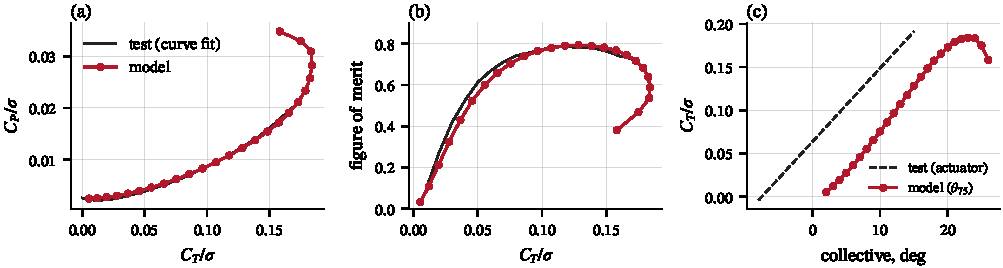
\includegraphics[width=\textwidth]{hover.pdf}
\caption{The isolated XV-15 rotor in hover at a tip Mach number of 0.69 against NASA's full-scale test (TM-86833 figs.~13, 14, 17): (a) power
against thrust, (b) figure of merit, (c) thrust against collective (the test's from the actuator's position, the model's at 0.75\,$R$).}\label{fig:hover}
\end{figure*}
\begin{table}[t]
\centering\small
\caption{The isolated XV-15 rotor in hover: power and figure of merit at the model's thrust.}\label{tab:hover}
\Tab{hover}
\end{table}

From $C_T/\sigma=0.08$ to 0.18 the rotor needs \NHcpMin{} to $+$\NHcpMax\,\% of the test's power at the same thrust (Fig.~\ref{fig:hover},
Table~\ref{tab:hover}), the figure of merit peaking at \NHfmMod{} at $C_T/\sigma=\NHfmCt$ against the test's 0.79 at 0.12, and the rotor reaches
$C_T/\sigma=\NHctMax$ at \NHthStall$^\circ$ of collective, where the test, which stopped at \NHctMaxTest, did not go. The sections' stall was
fitted here, so this checks the shape of the curve rather than predicts it. Below $C_T/\sigma=0.075$ the model needs \NHcpLowMin--\NHcpLowMax\,\%
more power than the test, more the lower the thrust: the profile power of the inboard sections, whose thick XN-like stand-ins have more drag
at low lift than the 64-series. The thrust's gradient against collective is \NHgrad{} per degree against the test's \NHgradTest{} (\NHgradPct\,\%
steeper): the test's collective is the actuator's, which includes the blades' elastic twist under load, which the rigid blades do not have. Past the
maximum thrust the blades stall progressively and the gimbal whirls by a few degrees; the model's power there (the points that turn back in
Fig.~\ref{fig:hover}a) has no test to compare with.

\subsection{XV-15 level-flight power}\label{sec:xv15}
\begin{figure*}[t]
\centering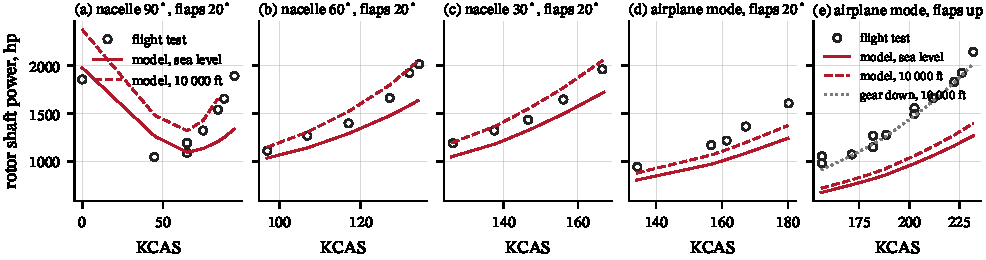
\includegraphics[width=\textwidth]{xv15.pdf}
\caption{XV-15 rotor shaft power in level flight against the flight test (TM-84222 fig.~20) at 13\,000\,lb: the model at sea level and at 10\,000\,ft,
which bracket the test's unpublished altitudes, gear up; in (e) also with the gear down.}\label{fig:xv15}
\end{figure*}
\begin{table}[t]
\centering\small
\caption{XV-15 level-flight power, model/test $-1$ at the test's points.}\label{tab:xv15}
\Tab{xv15}
\end{table}

Through the conversion, nacelles at 60$^\circ$ and 30$^\circ$ with 20$^\circ$ of flap, the test lies between the model at sea level and at
10\,000\,ft (Fig.~\ref{fig:xv15}, Table~\ref{tab:xv15}): \NXsMin{} to \NXsMax\,\% and \NXcMin{} to \NXcMax\,\% at sea level, \NXsHiMin{} to \NXsHiMax\,\%
and \NXcHiMin{} to \NXcHiMax\,\% at 10\,000\,ft, as the test's altitudes would have it. In airplane mode the model needs less power than the test at
either altitude: \NXfMin{} to \NXfMax\,\% with 20$^\circ$ of flap at sea level and, flaps up, \NXaSlMin{} to \NXaSlMax\,\% at sea level and \NXaMin{} to
\NXaMax\,\% at 10\,000\,ft. With the gear extended, its 4\,ft$^2$ of drag~\cite{cr} brings the flaps-up power to \NXgMin{} to \NXgMax\,\% at 10\,000\,ft;
the test's gear position is not given, but in airplane mode it would have been up. Bell's airframe coefficients, from wind tunnel tests of the clean
model, miss part of the flying aircraft's drag; the V-22's needed 11.5\,ft$^2$ more to meet Boeing's polar for the same reason (Section~\ref{sec:polar}).
The XV-15 build keeps Bell's data as they are.

In helicopter mode the model's power falls too fast with speed: \NXhelLo\,\% at 45\,kt, \NXhelHi\,\% at 94\,kt at sea level, \NXhover\,\% in the
hover. Bell's own simulation used an empirical profile power for the rotor in this regime; the blade elements here give a translational lift that
lowers the induced power faster than the test, and the wing in the slipstream at a high angle of attack, with 20$^\circ$ of flap, sees the wake model's
velocities, whose sweep off the wing through the transition is not checked by any test.

\subsection{Download}\label{sec:download}
\begin{figure*}[t]
\centering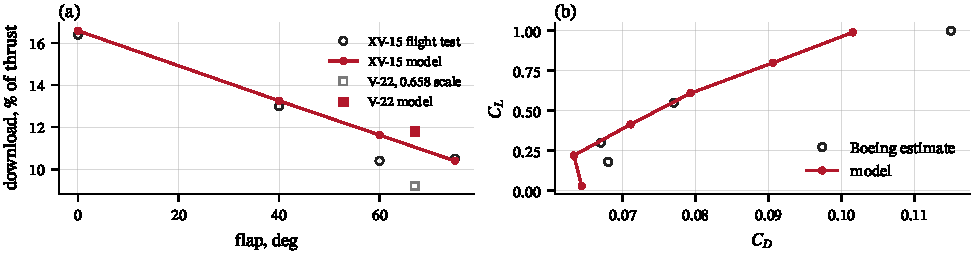
\includegraphics[width=0.72\textwidth]{download_polar.pdf}
\caption{(a) The wing's download in the hover against flap angle: the XV-15 (13\,300\,lb, flight test~\cite{rc} fig.~18) and the V-22 at 67$^\circ$
(0.658-scale rotor and wing test). (b) The V-22 airframe's lift and drag in airplane mode, flaps and gear up, against Boeing's full-scale estimate~\cite{rc} fig.~28.}\label{fig:dlpolar}
\end{figure*}
\begin{table}[t]
\centering\small
\caption{Download in the hover, \% of the rotors' thrust.}\label{tab:download}
\Tab{download}
\end{table}

The download factor of each of Bell's flap settings was fitted to the XV-15's flight-measured download, which the model then follows within
\NDlXmax{} point of thrust (Fig.~\ref{fig:dlpolar}a, Table~\ref{tab:download}). Carried to the V-22 with its own wing and rotors, at the hover's
67$^\circ$ of flaperon, it gives \NDlV\,\% against the 0.658-scale test's \NDlVtest\,\%: the V-22's flaperons, which fold down over a larger part of
the chord than the XV-15's flaps, take more of the wing out of the wake than the XV-15's tables know.

\subsection{V-22 airframe polar}\label{sec:polar}
\begin{table}[t]
\centering\small
\caption{V-22 airframe drag coefficient at Boeing's lift coefficients, on 382\,ft$^2$; $\Delta$ in drag counts.}\label{tab:polar}
\Tab{polar}
\end{table}
Bell's wing and empennage tables applied to the V-22's surfaces give it a lift coefficient of \NPclzero{} at zero angle of attack and a slope of
\NPslope{} per degree, against Boeing's 0.18 and about 0.093 (Fig.~\ref{fig:dlpolar}b, Table~\ref{tab:polar}). Its drag, with the 11.5\,ft$^2$ fitted
here, is \NPcdTwo{} at $C_L=0.2$ against 0.068; the model's polar is flatter than Boeing's estimate, whose drag rises faster beyond $C_L=0.6$.

\subsection{V-22 performance}\label{sec:perf}
\begin{figure*}[t]
\centering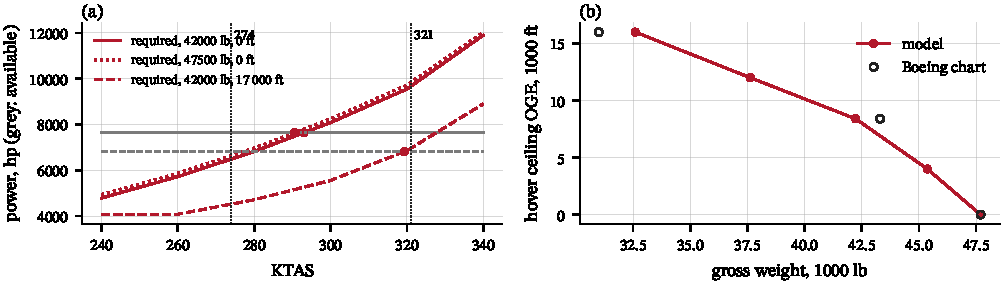
\includegraphics[width=\textwidth]{perf.pdf}
\caption{V-22 performance against Boeing's charts~\cite{rc} (standard day, 6150\,shp engines): (a) power required in airplane mode at 84\,\% rotor speed and
power available (grey: the engines' rating or the drive's torque limit, whichever is less); the dotted verticals are the chart's maximum speeds at
42\,000\,lb. (b) Hover ceiling out of ground effect at 100\,\% rotor speed.}\label{fig:perf}
\end{figure*}
\begin{table}[t]
\centering\small
\caption{V-22 performance, model and Boeing's charts.}\label{tab:perf}
\Tab{perf}
\end{table}

The drive's torque limit was fitted to the hover ceiling at sea level, 47\,700\,lb, where Boeing's chart has its knee: the transmission limits there,
the engines above. With it the ceiling is \NCmid\,lb at 8400\,ft (\NCmidPct\,\%) and \NChi\,lb at 16\,000\,ft (\NChiPct\,\%), where the engines' lapse
sets it (Fig.~\ref{fig:perf}, Table~\ref{tab:perf}). At 42\,000\,lb the maximum level speed is \NVsl\,KTAS at sea level against 274, limited by the drive's
torque at 84\,\% rotor speed, and \NVhi\,KTAS at 17\,000\,ft against 321, limited by the engines.

\subsection{The conversion}\label{sec:conv}
\begin{figure*}[t]
\centering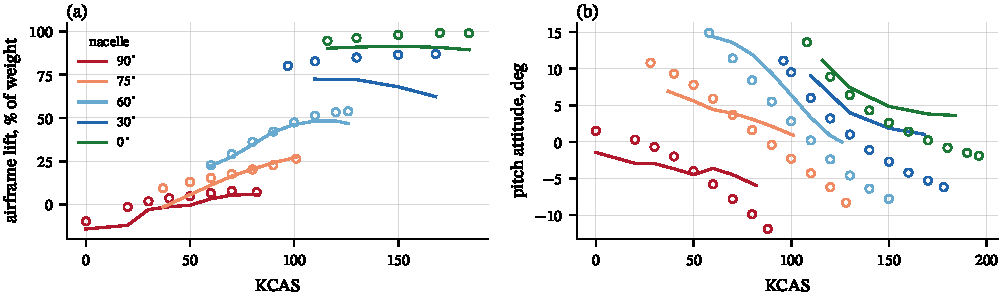
\includegraphics[width=\textwidth]{conversion.pdf}
\caption{Trims through the conversion at 34\,000\,lb, sea level, against the V-22's flight test~\cite{pd} figs.~7 and 9a: (a) the airframe's share of the
lift, (b) pitch attitude, by nacelle angle (circles: test).}\label{fig:conv}
\end{figure*}
\begin{table}[t]
\centering\small
\caption{Conversion, model minus test.}\label{tab:conv}
\Tab{conversion}
\end{table}
The pitch attitude follows the flight test through the conversion within \NCvPitchRms$^\circ$ (rms; Fig.~\ref{fig:conv}, Table~\ref{tab:conv}), the
model a few degrees nose-up of it at the higher speeds of each nacelle angle. The wing carries \NCvLiftRms\,\% of the weight less than Dunford's chart
(rms), most at 30$^\circ$ of nacelle, where the model's wing carries \NCvWingLo--\NCvWingHi\,\% against \NCvTestLo--\NCvTestHi\,\%: at that angle the rotors' slipstream over the wing, which
the wake model gives, decides the wing's lift, and no test checks it. The charts' weight and flaps are not published (Section~\ref{sec:ref}).

\subsection{Handling with the augmentation, and the start}\label{sec:handling}
\begin{figure*}[t]
\centering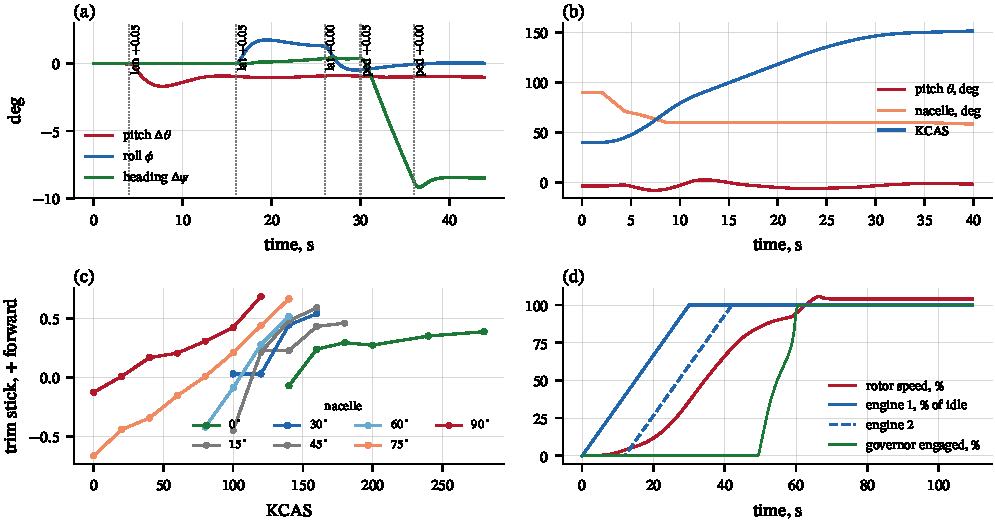
\includegraphics[width=\textwidth]{handling.pdf}
\caption{The FlightGear aircraft, augmentation on, reference loading: (a) single keyboard steps (5\,\% of travel) from the hover, stick centred; (b) a hands-off
conversion from 40\,kt, the nacelles commanded from 90 to 60$^\circ$; (c) the trim feed-forward, the level-flight trim's stick against airspeed by nacelle angle;
(d) an engine start on the ground, lever down.}\label{fig:handling}
\end{figure*}
These are not comparisons but checks of the FlightGear aircraft's augmentation (Fig.~\ref{fig:handling}). In the hover one press of the stick forward gives
\NHdTheta$^\circ$ of pitch, held, and one to the right \NHdPhi$^\circ$ of roll after a small overshoot; one of the pedals turns it at
\NHdYaw$^\circ$/s and the heading holds where they are let go. With the
nacelles commanded from 90 to 60$^\circ$ at 40\,kt and nothing else touched, the aircraft accelerates to \NCvEnd\,kt with its pitch between \NCthMin{} and
\NCthMax$^\circ$: the trim feed-forward takes up the trim's change, the stick's trim moving from \NTmAft\,\% of its travel aft of centre in the hover at
75$^\circ$ to \NTmFwd\,\% forward at 120\,kt at 90$^\circ$, which the bare aircraft would have the pilot hold. The nacelles stop at the corridor's lower boundary until the airspeed allows 60$^\circ$, and later move on
past it as the upper boundary comes down. Cold, with the lever down, the engines spool up one after the other and the rotors reach their governed speed
\NStNr\,s after the first engine's start.

\subsection{The hover hold}\label{sec:hoverhold}
\begin{figure*}[t]
\centering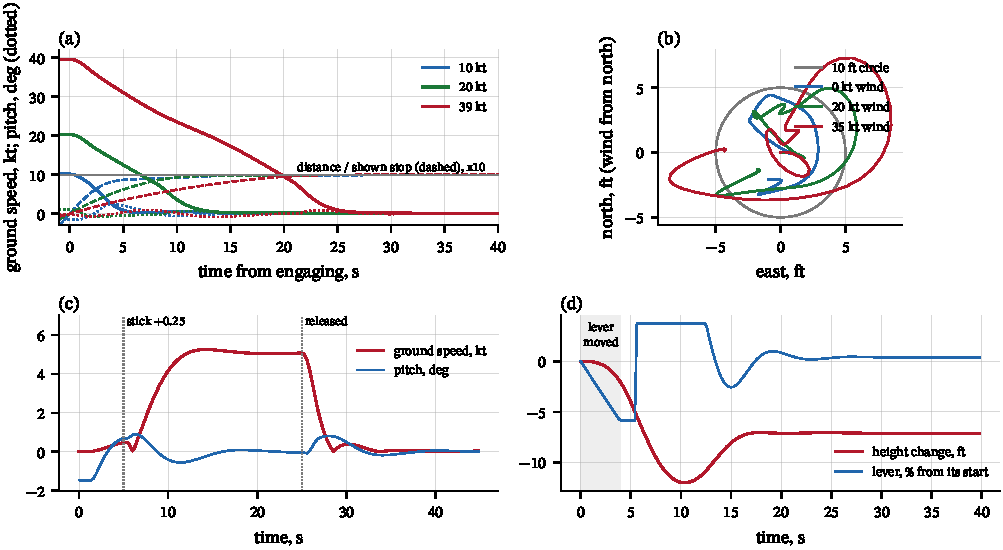
\includegraphics[width=\textwidth]{hover_hold.pdf}
\caption{The hover hold, reference loading, augmentation on: (a) engaged from 10, 20 and 39\,kt, the ground speed, the pitch attitude
(dotted) and the distance flown over the stop it showed (dashed); (b) ADS-33E-PRF's position hold check, a 360$^\circ$ turn on the pedals in
about 30\,s in a steady wind from the north, the track about the hold point; (c) the stick out of its detent and back; (d) the lever moved
down for 4\,s and left.}\label{fig:hoverhold}
\end{figure*}
The hover hold (HVR CPLD) follows the AH-64D's modern control laws~\cite{harding}, Bell's automatic hover hold~\cite{bellhh} and
ADS-33E's position hold and translational rate command~\cite{ads33}, with the V-22's own way of translating: on its nacelles, the
fuselage level~\cite{fsf}, as NASA's large tiltrotor's translational rate command does~\cite{malpica}. Engaged at up to 40\,kt over the ground, it sets the stop point, where the present velocity comes to rest at
0.08\,$g$, and flies one profile to it, then holds it and the height (radar height below 500\,ft, the barometric altitude above); the
nacelles take the fore and aft acceleration, the bank the sideways, the pitch only what is past the nacelles' range. Engaged at
\NHhStopV\,kt it stops \NHhStopD\,ft on, holding \NHhStopT\,s after; every stop ends within \NHhStopErr\,ft of the point it showed, the pitch
within \NHhStopPitch$^\circ$ (Fig.~\ref{fig:hoverhold}a). In ADS-33E's check, a turn on the pedals in about 30\,s, the aircraft stays within
\NHhTurnCalm\,ft of the point in still air, which meets the 10\,ft circle, \NHhTurnTwenty\,ft in 20\,kt of wind and \NHhTurnGale\,ft in 35\,kt, about
twice the circle's radius, its attitudes within \NHhTurnAttGale$^\circ$ against the 18$^\circ$ allowed (Fig.~\ref{fig:hoverhold}b). The stick out of
its detent commands a ground speed: \NHhTrcV\,kt for a quarter of its travel, reached to 63\,\% in \NHhTrcT\,s (2.5--5\,s), overshooting by
\NHhTrcOver\,kt, and on its release the aircraft stops and holds where it does (Fig.~\ref{fig:hoverhold}c). The hold drives the lever and
the pilot can fly through it: moved for 4\,s and left, the aircraft settles \NHhLeverDh\,ft lower, held within \NHhLeverHold\,ft
(Fig.~\ref{fig:hoverhold}d). The hold's sideways loop works through the roll attitude's, which needed twice its first gains; the 35\,kt
turn's errors come from the wind's loads turning with the aircraft faster than the hold's integrators follow.

% =====================================================================================================================
\section{Corrections found during validation}\label{sec:review}
The changes that the comparisons forced are listed here because each removed a physical or numerical inconsistency rather than tuning a coefficient.
\begin{enumerate}
\item \emph{The sections' stall.} The sections first had C-81's NACA 0012 stall, the lift falling to a flat plate's within 6$^\circ$. Its negative lift slope
past the maximum took away the gimbal's aerodynamic damping, and at high thrust the gimbal diverged. The 64-series sections stall from the trailing edge and fall
gently~\cite{nacar}; so do the model's now, the shape fitted to the hover test.
\item \emph{The nacelles' mass.} Each nacelle's centre of gravity was placed on the wrong side of the conversion axis, which put the aircraft's 5\,in forward.
\item \emph{The governor.} Its error had the wrong sign: a rotor slower than its reference took more collective, so it slowed further. And its engagement was
gated at an absolute rotor speed of 85--95\,\%, which turned it off in airplane mode at 84\,\%; it is gated relative to the reference now.
\item \emph{The flaperons in slow airplane mode.} Retracted with the nacelles down, they left the wing unable to carry the aircraft at the corridor's lowest
airplane-mode speeds; the schedule keeps 40$^\circ$ there.
\item \emph{Test weights.} The tests' weight changes went into the cargo's point mass, which moved the centre of gravity with them; they are at the design centre of
gravity now.
\item \emph{The drive's torque limit} was applied as a power proportional to the rotor speed, so a start had almost no torque to turn the rotors up; it acts as a
torque now, and the flight idle is the power the rotors need at flat pitch at their governed speed.
\item \emph{The gear in the comparisons.} The harness first ran with the gear extended, JSBSim's default. Its drag stood in for drag the airframe lacks: the V-22's
fitted drag (then 4.7\,ft$^2$) met Boeing's polar and the airplane-mode speeds only with the gear down, and the XV-15's airplane-mode power looked close. All comparisons
in forward flight are now gear up, the V-22's drag refitted, and the XV-15's shortfall reported (Section~\ref{sec:xv15}).
\item \emph{The nacelle rate.} The nacelles' tilt rate, which moves the hubs and adds to the shafts' pitch rate in the flapping, was taken after
the step had already set the new nacelle angle, so it was zero throughout. Taken from the step itself it changes no trim, and the pitch attitude
through the conversion run (Section~\ref{sec:handling}) by up to 1.6$^\circ$.
\item \emph{The handling runs' start.} The harness let the aircraft go one frame after setting the lever and centring the stick, before the
controls' chain (the mixing, its actuators, the governor) had carried them through, and set the augmentation's integrators from that frame's
values: the hover run began with a 2\,\% sag in rotor speed, drifted 3\,kt and lost 40\,ft that the aircraft does not. It now waits a whole
period of the controls' channels (four frames) before letting go, and the hover holds its rotor speed and height from the start.
\item \emph{The trim feed-forward in rearward flight.} The augmentation's trim feed-forward looked its stick up against the airspeed's
magnitude, so that flying backwards it gave the forward stick of forward flight: in FlightGear the aircraft let go in the hover drifted aft,
pitched nose down and diverged with the augmentation's integrator at its limit. It takes the forward airspeed now (the hover's stick in
rearward and sideward flight), carried past 90$^\circ$ of nacelle along its slope from 75 to 90.
\item \emph{Yaw at low speed.} The augmentation only damped the yaw rate, through a washout: a steady yaw moment, a tailwind on the fins,
turned the aircraft at will, and the pedals, opposed by the damper, were weak (a keyboard step turned it 0.6$^\circ$). Below 50\,kt the pedals
now command a yaw rate, held by an integrator with the pedals' full travel.
\end{enumerate}

% =====================================================================================================================
\section{Assessment}\label{sec:assess}
\begin{table}[t]
\centering\small
\caption{Summary: \ok{} within the test's scatter, \pok{} partly, \nok{} not reproduced. Fitted: the comparison checks the shape only.}\label{tab:score}
\begin{tabularx}{\columnwidth}{@{}>{\raggedright\arraybackslash}Xc@{}}
\toprule
XV-15 rotor: hover power, $C_T/\sigma=0.08$--0.18 (stall fitted) & \ok \\
XV-15 rotor: hover power at low thrust; collective gradient & \pok \\
XV-15 download against flaps (fitted) & \ok \\
XV-15 power through the conversion (altitudes bracketed) & \ok \\
XV-15 power in helicopter mode, 45--94\,kt & \nok \\
XV-15 power in airplane mode, gear up (Bell's drag) & \nok \\
V-22 airframe polar (drag fitted) & \ok \\
V-22 maximum level speed, sea level and 17\,000\,ft & \ok \\
V-22 hover ceiling (sea level fitted) & \ok \\
V-22 download at 67$^\circ$ & \pok \\
V-22 pitch attitude through the conversion & \ok \\
V-22 wing lift share through the conversion & \pok \\
\bottomrule
\end{tabularx}
\end{table}
Table~\ref{tab:score} summarises. The model reproduces what defines the tiltrotor's performance: the proprotor's hover power at operating thrust, the
wing's download against its flaps, the airframe's polar, and the V-22's speeds and hover ceilings, the last three after one fitted drag area and one
fitted torque limit, both against Boeing's own charts. Through the conversion the V-22's pitch attitude follows its flight test. Its open items are the
helicopter mode's power against speed, where the XV-15's test shows a shallower bucket than the blade elements and the wake give; the drag Bell's
coefficients lack, which the V-22 build supplies by a fit and the XV-15 build leaves; the wing's share of the lift at intermediate nacelle angles; and
the V-22 wing's download. None of the V-22's dynamic responses could be compared: no frequency responses or time histories of the aircraft are public, and
the XV-15's, which are~\cite{tis}, are left for further work. Its augmentation is a plausible control law, not the V-22's.

% =====================================================================================================================
\section{Conclusions}\label{sec:concl}
\begin{itemize}
\item A blade-element model of the gimballed tiltrotor, both rotors blade by blade with their gimbals, pitch--flap coupling and finite-state wakes, the
wing in their ring-vortex wakes, the interconnected drive and the conversion corridor, runs in plain JSBSim, generated from data. It is the flight
model of the FlightGear V-22.
\item Built first as the XV-15 from Bell's simulation data and NASA's tests, its rotor gives the full-scale rotor's hover power at operating thrust, and
its download follows the flight test's with the flap.
\item Carried to the V-22 with its published data, one fitted drag area and one fitted torque limit, it gives Boeing's airframe polar, maximum speeds
within 15\,kt and hover ceilings within 5\,\%, and the flight test's pitch attitude through the conversion.
\item Bell's airframe coefficients miss part of the flying aircraft's drag; with the gear up the XV-15 build needs a quarter to a third less power than
its flight test in airplane mode.
\item The helicopter mode's power against speed, the wing's lift through the middle of the conversion and the V-22's download are documented, not tuned away.
\end{itemize}

\begin{thebibliography}{99}\small
\bibitem{cr} H.\ Harendra, M.\ Joglekar, T.\ Gaffey and R.\ Marr, \emph{V/STOL Tilt Rotor Study, Volume V: A Mathematical Model for Real Time Flight Simulation of the Bell Model 301 Tilt Rotor Research Aircraft}, NASA CR-114614, 1973.
\bibitem{tx} NASA/Army Tilt Rotor Project Office, \emph{Tilt Rotor Research Aircraft Familiarization Document}, NASA TM X-62407, 1975.
\bibitem{fb} F.\,F.\ Felker, M.\,D.\ Betzina and D.\,B.\ Signor, \emph{Performance and Loads Data from a Hover Test of a Full-Scale XV-15 Rotor}, NASA TM-86833, 1985.
\bibitem{cd} G.\,B.\ Churchill and D.\,C.\ Dugan, \emph{Simulation of the XV-15 Tilt Rotor Research Aircraft}, NASA TM-84222, 1982.
\bibitem{ma} M.\,D.\ Maisel, D.\,J.\ Giulianetti and D.\,C.\ Dugan, \emph{The History of the XV-15 Tilt Rotor Research Aircraft: From Concept to Flight}, NASA SP-2000-4517, 2000.
\bibitem{rc} H.\ Rosenstein and R.\ Clark, \emph{Aerodynamic Development of the V-22 Tilt Rotor}, 12th European Rotorcraft Forum, paper 14, 1986.
\bibitem{pd} P.\ Dunford, K.\ Lunn, R.\ Magnuson and R.\ Marr, \emph{The V-22 Osprey -- a Significant Flight Test Challenge}, 16th European Rotorcraft Forum, paper II.7.3, 1990.
\bibitem{ac} C.\,W.\ Acree, \emph{Assessment of JVX Proprotor Performance Data in Hover and Airplane-Mode Flight Conditions}, NASA/TM-2016-219070, 2016.
\bibitem{wj} W.\ Johnson, \emph{Airloads and Wake Geometry Calculations for an Isolated Tiltrotor Model in a Wind Tunnel}, American Helicopter Society, 2001.
\bibitem{fs} Naval Air Systems Command, PMA-275, \emph{V-22 Osprey Fact Sheet}, about 2001.
\bibitem{gs} GlobalSecurity.org, \emph{V-22 Osprey: fuel system}.
\bibitem{nacar} I.\,H.\ Abbott, A.\,E.\ von Doenhoff and L.\,S.\ Stivers, \emph{Summary of Airfoil Data}, NACA Report 824, 1945.
\bibitem{heyson} H.\,H.\ Heyson, \emph{Ground Effect for Lifting Rotors in Forward Flight}, NASA TN D-234, 1960.
\bibitem{hk} H.\,H.\ Heyson and S.\ Katzoff, \emph{Induced Velocities Near a Lifting Rotor with Nonuniform Disk Loading}, NACA Report 1319, 1957.
\bibitem{ph} D.\,A.\ Peters and C.\,J.\ He, \emph{Finite State Induced Flow Models, Part II: Three-Dimensional Rotor Disk}, Journal of Aircraft 32(2), 1995.
\bibitem{metu} Middle East Technical University, M.Sc.\ thesis on forward flight trim and longitudinal stability codes (Peters--He finite-state wake equations).
\bibitem{ads33} US Army Aviation and Missile Command, \emph{Aeronautical Design Standard Performance Specification, Handling Qualities
Requirements for Military Rotorcraft}, ADS-33E-PRF, 2000.
\bibitem{harding} J.~W. Harding, M.~H. Mansur, M.~B. Tischler, S.~J. Moody and R.~C. McCann, \emph{Optimization and Piloted Simulation
Results of the AH-64D Modern Control Laws}, AHS 63rd Annual Forum, 2007.
\bibitem{malpica} C.~A. Malpica, B. Lawrence, J. Lindsey, C.~R. Theodore and C.~L. Blanken, \emph{Handling Qualities of a Large Civil
Tiltrotor in Hover using Translational Rate Command}, AHS 68th Annual Forum, 2012.
\bibitem{bellhh} Bell Helicopter Textron, \emph{Flight control laws for automatic hover hold}, US patent application 2013/0138270, 2013.
\bibitem{fsf} Flight Safety Foundation, \emph{Helicopter Safety}, November--December 1988 (the V-22's handling in VTOL mode).
\bibitem{patent} Boeing, \emph{Control law mode switching between rate command and attitude command control systems}, US patent 5\,596\,499, 1997.
\bibitem{tis} M.\,B.\ Tischler, J.\,G.\,M.\ Leung and D.\,C.\ Dugan, \emph{Identification and Verification of Frequency-Domain Models for XV-15 Tilt-Rotor Aircraft Dynamics}, NASA TM-86009, 1984.
\bibitem{jsbsim} JSBSim Development Team, \emph{JSBSim: an open-source flight dynamics model}, version 1.3.3.
\end{thebibliography}
\end{document}
